\addbibresource{reference.bib}

\chapter{Úvod do hybridních částicových pixelových detektorů}\label{chap:detectors}
Ionizující záření je lidskými smysli nedetekovatelné, avšak jeho studie nám umožňuje pochopit podstatu hmoty, její vlastnosti a interakce. To lidstvu umožnilo mnohé aplikace, jako je například protonová terapie \cite{tpx_app_radiotherapy}, defektoskopie nebo zkoumání pravosti uměleckých děl. První pokusy o detekci ionizujícího záření sahají do počátku 20. století, kde pomocí mlžné komory se prvně podařilo zachytit trajektorii nabitých částic. Rozvoj polovodičové technologie dal vzniku novým detekčním technologiím až po v současné době nejpokrokovějším - pixelovým detektorům.

Existuje celá řada částicových pixelových detektorů, ale v této kapitole budou popsány jen hybridní pixelové detektory, pro které je typické, že se skládají ze dvou nezávisle vyrobených částí - senzoru a vyčítacího čipu. To oproti monolitickým detektorů, kde vyčítací elektronika je součástí senzoru přináší řadu výhod, jako například snížení výrobních nákladů nebo možnost kombinace vyčítacího čipu se senzory různých materiálů (\textit{Si}, \textit{GaAs}, \textit{CaTe} apod.) a tlouštěk (vetšinou $300\mu m$, nebo $500\mu m$).

Na tomto místě je třeba zmínit, že existuje více druhů těchto detektorů (\textit{AGH Fermilab, Pilatus, Philips Chromaix} apod.)\cite{detectors_review}, v této práci budou použity použity pouze detektory z rodiny detektorů Medipix.

%********************************************************************************
% Hardwarová architektura
%********************************************************************************
\section{Hardwarová architektura}
\begin{figure}[th]
	\begin{center}
		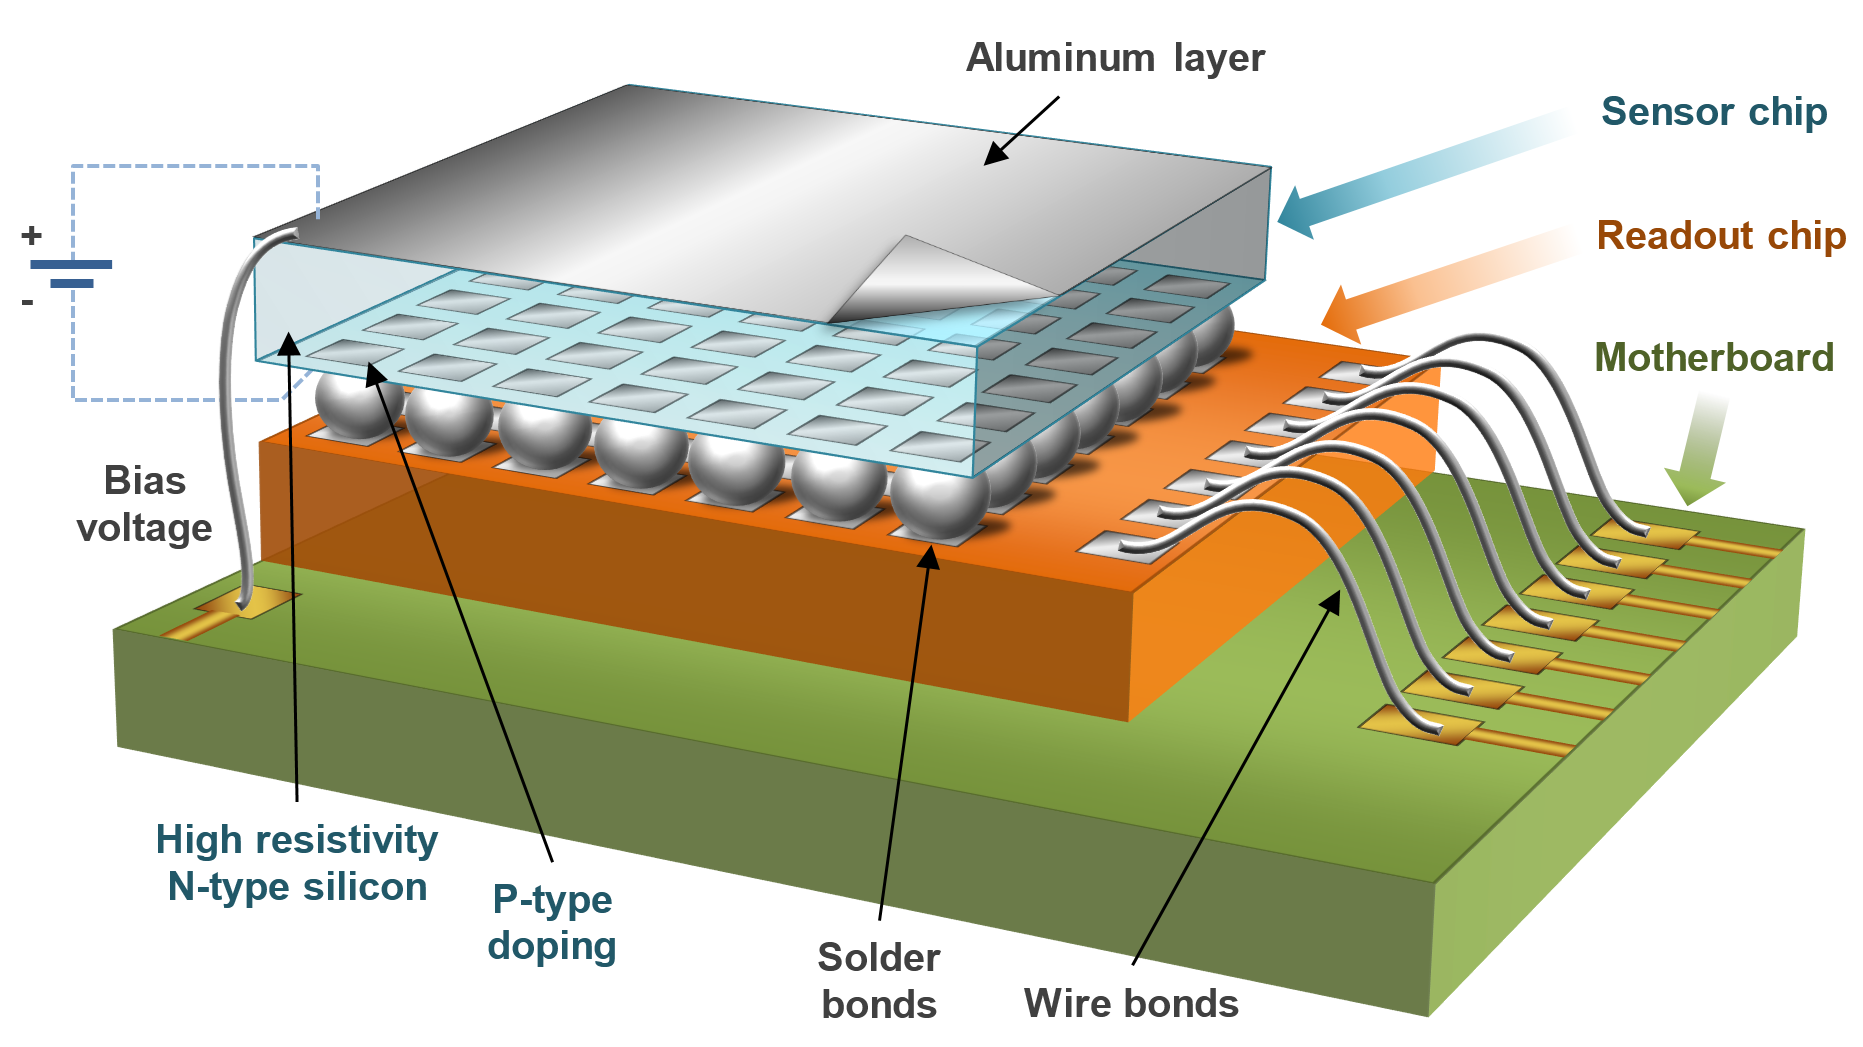
\includegraphics[width=12cm]{figures/det_chip.png}
		\caption{Struktura hybridního polovodičového pixelového detektoru Timepix3, skládající se z vyčítacího čipu a polovodičového senzoru \cite{PlatkevicDisertace}.}
		\label{fig:det:chip}
	\end{center}
\end{figure}
Většina hybridních částicových pixelových detektorů rodiny Medipix obsahuje matici $256\times256$ pixelů. Každý z nich má stanu o délce $55~\mu m$, takže senzor čítající $65536$ má plochu $1.4 \times 1.4 cm^2$. 

Na obrázku \ref{fig:det:chip} je znázorněna struktura detektoru Timepix3. Vrchní část detektoru tvoří polovodičový senzor, který je nejčastěji vyroben z křemíku, ale výjimkou není také \textit{GaAs} nebo \textit{CaTe}. Jednotlivé pixely senzoru jsou spojeny s integrovaným \texttt{ASIC}\footnote{z angl. Application Specific Integrated Circuit} vyčítacím čipem pomocí technologie zvané \textit{Bump-Bounding}. Vyčítací čip je pak propojen se základní deskou pomocí \textit{wire-bound}, z které je ještě přivedeno měřící napětí na senzor detektoru (tzv. \textit{bias}).


%********************************************************************************
% Princip detekce
%********************************************************************************
\section{Princip detekce}\label{chap:detectors:princip}
\begin{figure}[th]
	\begin{center}
		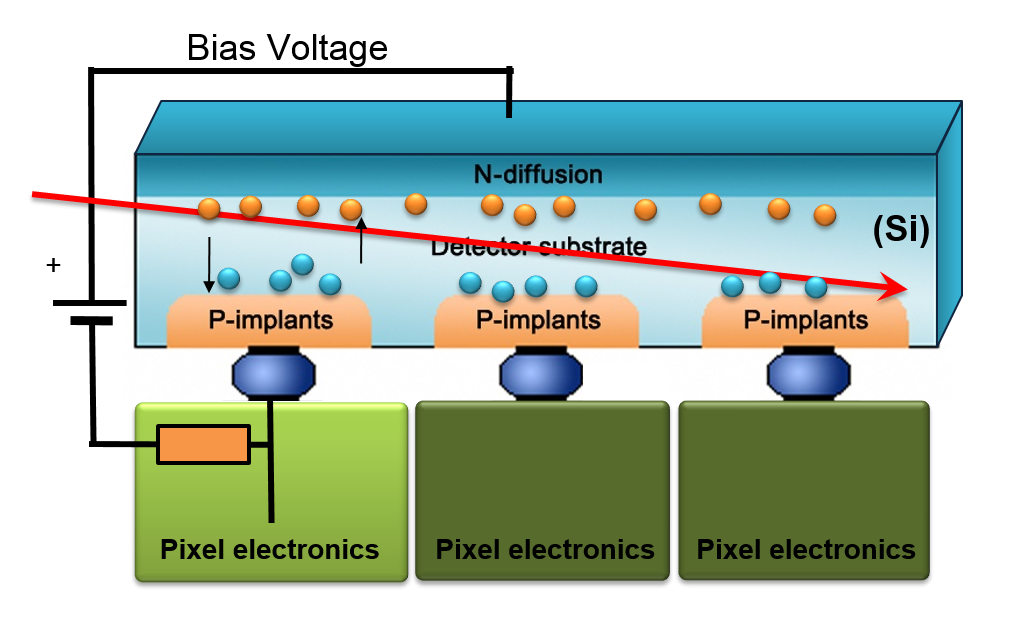
\includegraphics[width=10cm]{figures/det_recombination.png}
		\caption{Princip detekce ionizujícího záření detektorem Timepix3 \cite{PlatkevicDisertace}.}
		\label{fig:det:recombination}
	\end{center}
\end{figure}

Princip detekce ionizujícího záření pixelovými detektory je založen na známém jevu detekce ionizujícího záření v polovodiči. 

Jako náhradní schéma jednoho pixelu si lze představit diodu zapojenou v závěrném směru, kterou bez přítomnosti ionizujícího záření protéká minimální proud. Vnikne-li do senzoru ionizující částice a dojde k její interakci se senzorem, resp. část její energie je deponována do polovodičového objemu senzoru, dojde v senzoru ke vzniku elektron-děrových páru a díky lavinovému efektu i k následnému otevření PN přechodu (viz. na obr. \ref{fig:det:recombination}, kde červená šipka znázorňuje interagující částici, elektrony jsou znázorněny žlutě, modře díry).

Vzniklý proudový impulz je měřícím odporem převeden na napětí, které je komparátorem porovnáno s prahovým napětím (tzv. \textit{threshold}). Výsledek této komparace je dále CMOS obvodem zpracován, dle použitého měřícího módu, jak bude ukázáno v kapitole \ref{chap:detectors:operation_modes}.

Na rozdíl od CCD technologii, CMOS readout \textit{Timepix}/\textit{Medipix} detektorů negeneruje temný proud\footnote{Termín charakterizující vyčítací šum u CCD snímačů. Obvykle je udáván v elektronech za sekundu při konstantní teplotě a ve tmě.}, díky odstínění signálu od šumu pomocí komparačního napětí. To znamená, že doba jedné akvizice je teoreticky neomezena, protože detektor je schopný detekovat jen ty částice, jejíchž deponovaná energie (resp. amplituda vzniklého napěťového pulzu) je větší, než \textit{threshold}.

%********************************************************************************
% Operační módy detektoru
%********************************************************************************
\section{Operační módy detektoru}\label{chap:detectors:operation_modes}
\begin{figure}[th]
	\begin{center}
		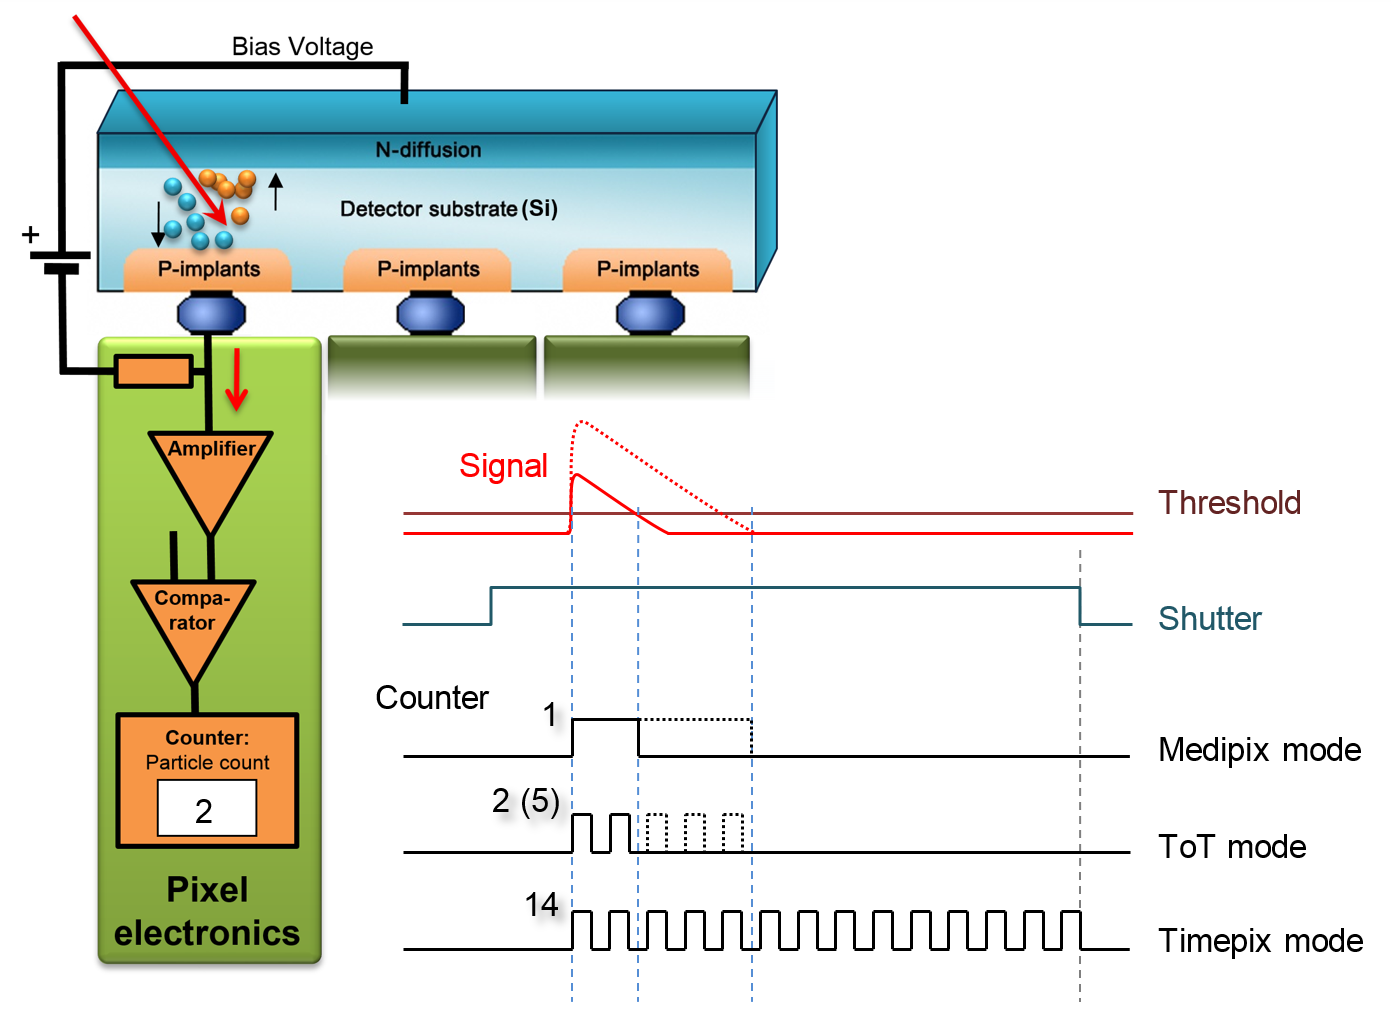
\includegraphics[width=14cm]{figures/det_pix.png}
		\caption{Zpracování signálu pixelem detektoru dle nastaveného módu (\textit{Medipix}, \textit{ToT} a \textit{ToA}) \cite{PlatkevicDisertace}.}
		\label{fig:det:modes}
	\end{center}
\end{figure}


V této podkapitole bude vysvětlena většina operačních módu, ve kterých detektory rodiny \textit{Medipix} jsou schopny pracovat. 

Jak už bylo popsáno v předchozí kapitole, interagovaná částice vyvolá napěťový impulz, jehož tvar koreluje s deponovanou energií. Pro účely analýzy se ale používá pouze binární informace o překročení prahového napětí v čase. Výsledek této analýzy je po jejím dokončení uložen ve 14-bitovém registru pixelu.

Na obr. \ref{chap:detectors:operation_modes} je znázorněn příklad zpracování analýzy signálu následujícími módy:
\begin{description}
    \item[Medipix mód (Counting mód)] V tomto módu je čítač inkrementován v každém cyklu měřící frekvence, pokud měřící napětí překročilo prahové napětí pixelu. Na konci akvizice pak hodnota čítače odpovídá počtu zaznamenaných částic.
    \item[Time-Over-Threshold (ToT)] Pracuje-li pixel v tomto módu, pak jeho čítač je inkrementování v každém cyklu měřící frekvence, pokud měřící napětí je vyšší, než prahové napětí pixelu. Hodnota uložená v čítači odpovídá deponované energii interagovaných částic. Mezi energií a \texttt{ToT} je nelineární závislost a její zkoumání je předmětem energetické kalibrace detektoru, jak bude ukázáno v kapitole \ref{chap:detectors:calibration:energy}. Tento mód má široké spektrum aplikací, například \cite{tot_app_counting} nebo \cite{tpx_app_radiotherapy}.
    \item[Time-of-Arrival (ToA)] Tímto módem disponují pouze detektory \textit{Timepix} a \textit{Timepix3}, avšak nesdílí stejný princip. Zatímco \textit{Timepix} detektor začne inkrementovat čítač v každém cyklu měřící frekvence po první náběžné hraně z komparátoru, \textit{Timepix3} na náběžnou hranu uloží do 14-bitového registru aktuální časové razítko z hodin detektoru. V obou případech \texttt{ToA} udává čas první interakce částice v dané akvizici.
\end{description}

%********************************************************************************
% Vyčítání naměřených dat
%********************************************************************************
\section{Vyčítání naměřených dat}\label{chap:detectors:readout}
Jednotlivé detektory rodiny \textit{Medipix} mají různou hardwarovou podporu pro vyčítání naměřených dat. Detektory vždy podporují alespoň jeden z těchto módů:
\begin{description}
	\item[Frame-Based] Pracuje-li detektor v tomto módu, pak jsou všechny registry čítačů pixelů vyčítány najednou, po dokončení aktuálního snímku. Vždy je třeba vyčíst všechny pixely bez ohledu na naměřenou hodnotu.
	\item[Data-Driven] Tento mód, také označovaný jako \textit{Event-Driven}, byl prvně použit v detektoru \textit{Timepix3}. Pracuje-li detektor v tomto módu, pak v průběhu akvizice dat (resp. když \textit{shutter} signál na nastaven na úroveň \texttt{HIGH}) každý pixel po zpracování události notifikuje readout interface o tom, že nová data jsou připravena k vyčtení a readout interface je pak bez prodlení vyčte a dále zpracuje.
\end{description}

Na obrázku \ref{fig:det:frame_vs_event_driven} je vidět hlavní motivace pro zavedení podpory \textit{Data-Driven} módu u detektoru \textit{Timepix3}. Ukázalo se, že \textit{Data-Driven} mód je efektivnější při takových měření, kde okupance snímků je menší než zhruba $50\%$. Po překročení této meze je efektivnější použití \textit{Frame-Based} módů, protože není třeba přenášet souřadnice zasažených pixelů. Podle \cite{timepix3} vyčítací čas může být definován následovně:
\begin{equation}\label{eq:det:readout_time}
	T_{readout} = N_{pixels}*bits_{pixel}/BW
\end{equation}
kde:
\begin{changemargin}{1.5cm}{1cm} 
	\begin{itemize}
		\item[$N_{pixels}$] je počet pixelů které je potřeba vyčíst (pro \textit{Frame-Based} mód jsou to všechny pixely detektoru ($256\times256$) a pro \textit{Data-Driven} je to počet zasažených pixelů),
		\item[$bits_{pixel}$] je počet bitů na pixel ($28 b$ v \textit{Frame-Based} módu a $28b + 16b$ v \textit{Data-Driven} módu kvůli nutnosti přenášení adresy pixelu) a
		\item[$BW$] je počet bytů za vteřinu, které je možné vyčíst z detektoru (\textit{bandwidth}). 
	\end{itemize}
\end{changemargin}

\begin{figure}[th]
	\begin{center}
		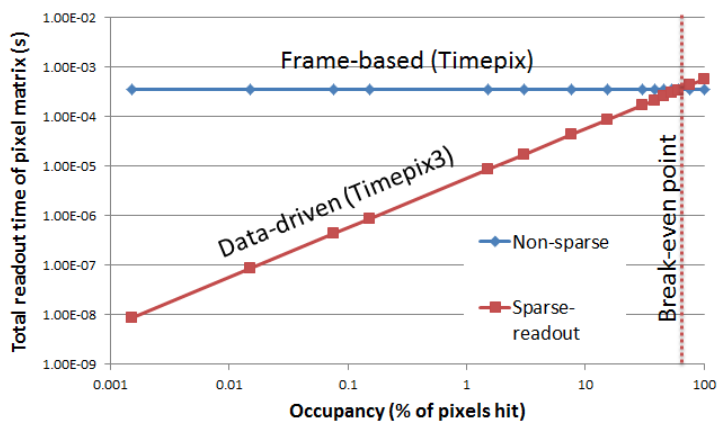
\includegraphics[width=14cm]{figures/det_frame_vs_event_driven.png}
		\caption{Doba vyčítání detektoru za použití \textit{Frame-based} (non-sparse) a \textit{Data-driven} (sparse) módu \cite{timepix3}.}
		\label{fig:det:frame_vs_event_driven}
	\end{center}
\end{figure}

%********************************************************************************
% Kalibrace
%********************************************************************************
\section{Kalibrace}\label{chap:detectors:calibration}
Každý detektor má své specifické vlastnosti, které jsou dány nejenom výrobním procesem, ale i závislostí na opotřebení a únavě materiálu v čase, okolní teplotě nebo na nastavených měřících parametrech (například \textit{bias}). Hlavní motivací pro kalibraci detektorů je minimalizace systematické chyby měření. Z pohledu aplikace získaných kalibračních dat je možné kalibrační metody rozdělit do dvou kategorií:
\begin{enumerate}[label=(\roman*)]
	\item Použití v průběhu akvizice dat - jedná se o data, která jsou použita pro nastavení akvizice dat v detektoru a mají přímý vliv na naměřená data, která danou metodou není možné dodatečně kalibrovat. Do této kategorie spadá například \textit{treshold equalizace} (viz \ref{chap:detectors:calibration:equalization}).
	\item Transformace naměřených dat - v tomto případě jsou kalibrační data aplikovaná dodatečně na naměřená data. Tento přístup má výhodu v možnosti dodatečné kalibrace již naměřených dat. To této kategorie spadá například \textit{Energetická kalibrace} (viz \ref{chap:detectors:calibration:energy}) nebo \textit{Time-Walk korekce} (viz \ref{chap:detectors:calibration:timeWalk}).
\end{enumerate}

\subsection{Treshold equalizace}\label{chap:detectors:calibration:equalization}
V podkapitole \ref{chap:detectors:princip} a \ref{chap:detectors:operation_modes} již bylo vysvětleno použití prahového napětí (\textit{treshold}) v průběhu akvizice dat detektorem. Každý pixel detektoru má ale rozdílné fyzikální vlastnosti dané výrobním procesem, s čímž souvisí i citlivost (resp. oddělení užitečného signálu od šumu) jednotlivých pixelů. Kromě globální hodnoty tresholdu je možné pro každý pixel upravit citlivost pomocí lokální $4b$ hodnoty tresholdu (viz obr. \todo přidat ref na schéma). 

Vlastní proces equalizace probíhá tak, že se udělá treshold scan přes všechny hodnoty, přičemž je třeba minimalizovat interakce detektoru z částicemi. V běžné praxi stačí detektor dostatečně odstínit. Výstupem tohoto procesu je pak globální treshold a jeho 4-bitové korekce pro jednotlivé pixely.

Jako vedlejší produkt tohoto procesu je rovněž maskovací matice detektoru, které obsahuje šumějící, nebo jinak poškozené pixely. To jsou například takové pixely, které bez přítomnosti interagujících částic hlásí překročení tresholdu.

\subsection{Energetická kalibrace}\label{chap:detectors:calibration:energy}
\begin{figure}[th]
	\begin{center}
		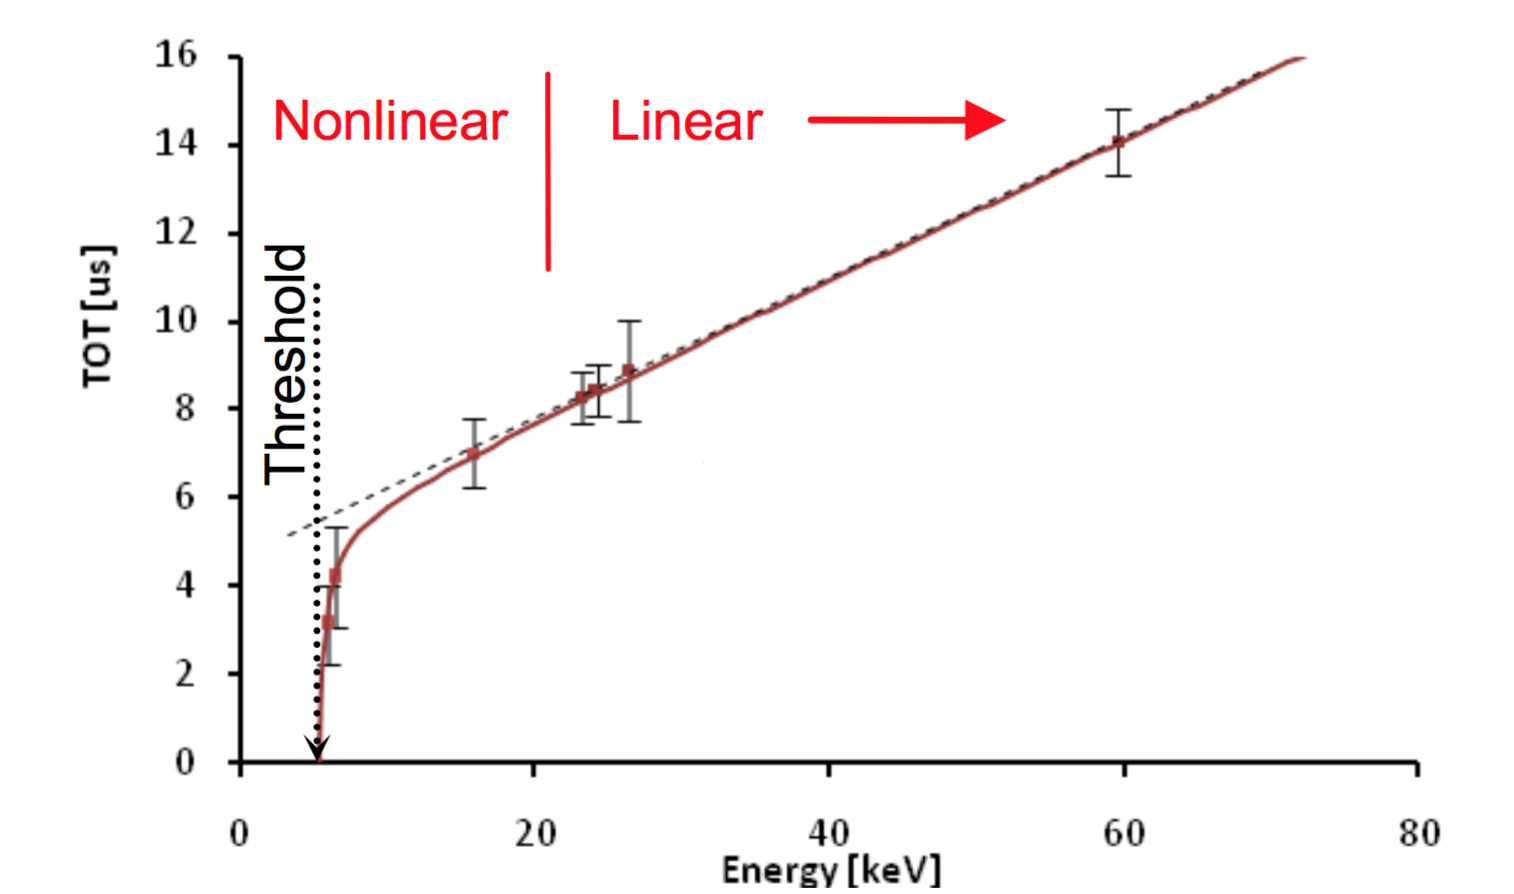
\includegraphics[width=13cm]{figures/calib_function.png}
		\caption{Kalibrační funkce, udávající závislost mezi energií v \texttt{keV} a \texttt{ToT} \cite{Jakubek2011S262}, vzniklá proložením získaných kalibračních bodů funkcí \ref{eq:det:energyCalib} a sestávající se ze dvou částí - (i) nelineární částí pro oblast nižších energií (hyperbola) a (ii) lineární částí pro vyšší energie (přijímka).}
		\label{fig:det:calib:calib_function}
	\end{center}
\end{figure}

V předchozí části práce byl již představen \textit{Time-Over-Treshold} mód (viz \ref{chap:detectors:operation_modes}), ve kterém je detektor schopný měřit deponovanou energii interagovaných v částic, která je udávána v \texttt{ToT}. Jak již bylo ukázáno, vztah mezi energií v \textit{keV} a \texttt{ToT} je nelineární závislost a závisí na fyzikální vlastnostech daného pixelu, což je předmětem energetické kalibrace, která bude v této podkapitole popsána.

Tato metoda \cite{Jakubek2011S262} spočívá v provedení několika sad měření se zdroji ionizujícího záření, jejichž energie jsou předem známy, a v jejich analytickém zpracování a vytvoření kalibrační funkce \ref{eq:det:energyCalib} pro každý pixel detektoru. V předchozí (bakalářské) práci \cite{BegeraBcThesis2016} byly tyto metody podrobně popsány a byl vytvořen software, který uživateli umožňuje vytvoření energetické kalibrace detektoru z naměřených dat.

\begin{equation}\label{eq:det:energyCalib}
	f_{calib}(x) = ax + b - \frac{c}{x-t}
\end{equation}

Pro měření kalibračních dat se jako efektivní řešení v praxi ukázalo použití rentgenové fluorescence\footnote{Děj ke kterému dochází při ozařování materiálu (nejčastěji \textit{Cu}, \textit{Fe}, \text{In} apod.) rentgenovým zářením, při kterém jsou z něj vyráženy excitované elektrony. Při vyražení elektronu na nižší energetické úrovni, elektron z vyšší energetické úrovně obsadí jeho místo a přebytečnou energii emituje formou vyzářeného fotonu - fluorescenčního záření, jehož charakteristické monoenergetické spektrum je pro většinu prvků dobře známé.} \cite{Jakubek-radiography_and_charge_sharing}. Pro zajištění dobré kvality kalibrace je třeba naměřit takový počet událostí, aby spektra ve snímcích byla dobře rozeznatelná. Z naměřeních dat jsou vyfiltrovány pouze tzv. \textit{Single-hit} události\footnote{Události, ve kterých částice interagovala pouze s jedním pixelem detektoru}, aby se minimalizovaly negativní vlastnosti \textit{Charge-sharing} efektu (díky společné elektrodě senzoru jsou díky interagující částici vzniklé elektrony zpracovány více pixely najednou a část deponované energie nemusí být ASIC čipem zpracována, protože vzniklý signál může být nižší než treshold daného pixelu).

\begin{figure}[th]
	\begin{center}
		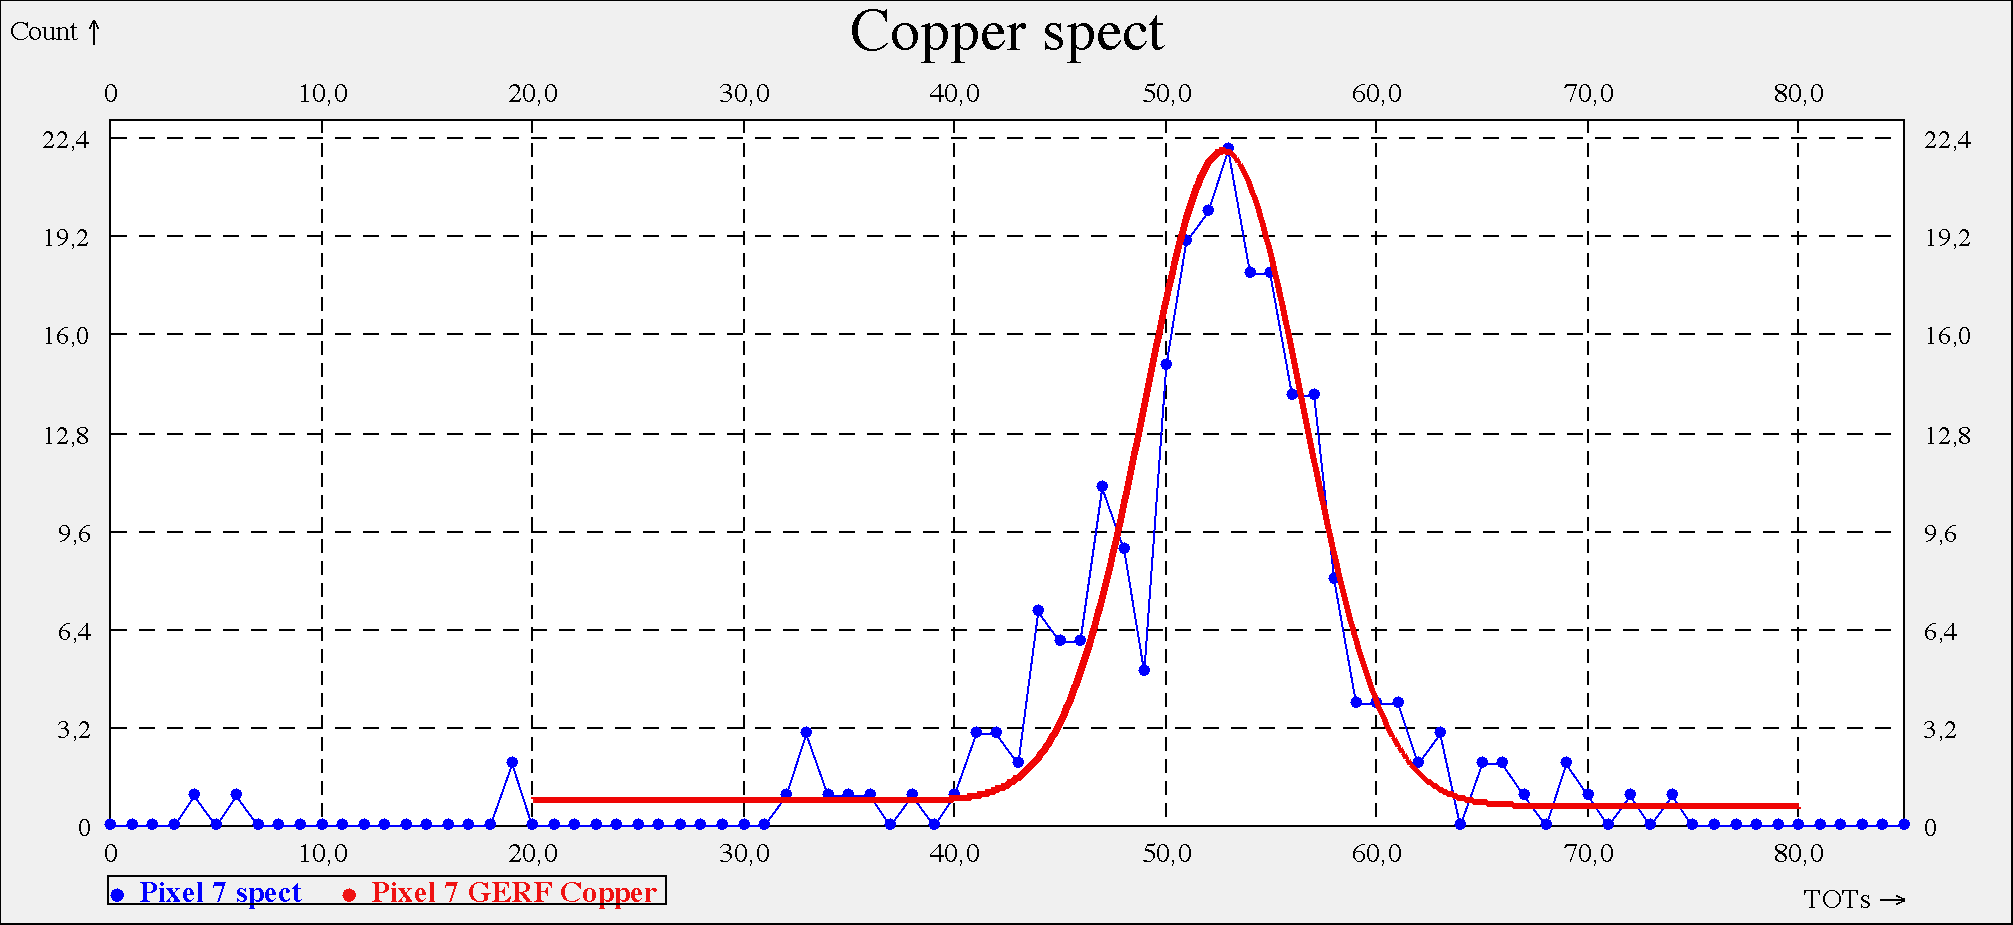
\includegraphics[width=15cm]{figures/calib_gerf.png}
		\caption{Příklad energetického spektra jednoho pixelu Timepix detektoru s proloženou funkcí \ref{eq:det:gerf} \cite{BegeraBcThesis2016}.}
		\label{fig:det:calib:gerf}
	\end{center}
\end{figure}

Z jednotlivých měření jsou pro každý pixel detektoru vytvořena spektra \texttt{ToT} hodnot. Na obrázku \ref{fig:det:calib:gerf} je znázorněn příklad takového spektra, získaného z fluorescence mědi. Požadovaný kalibrační bod se získá střední hodnoty \texttt{ToT} a tabulkové hodnoty energie fluorescenčního záření mědi. Střední hodnota je získána proložením spektra funkcí \ref{eq:det:gerf} - jedná se o součet Gaussovy funkce a Gaussovy chybové funkce (kvůli levé nesymetrii vzniklé \textit{Charge-sharing} efektem).

\begin{equation}\label{eq:det:gerf}
	f_{GERF}(x) = \underbrace{Ae^{ -\frac{(x-\mu)^2}{2\sigma^2} }}_{\text{Gaussova funkce}} +
	\underbrace{ \frac{avg_{right} - avg_{left}}{\sigma\sqrt{2\pi}} \int_{-\infty}^t e^{ -\frac{(t-\mu)^2}{2\sigma^2} } + avg_{left}}_{\text{Gaussova chybová funkce}}
\end{equation}
kde:
\begin{changemargin}{1.5cm}{1cm} 
	\begin{itemize}
		\item [$A$] je amplituda,
		\item [$\mu$] je stření hodnota hledané energie,
		\item [$\sigma$] je rozptyl střední hodnoty energie $\mu$, který je možné vypočítat ze vzorce 
			\ref{eq:det:gerf_sigma}, kde \texttt{FWHM}\footnote{z angl. Full Width at Half Maximum} udává šířku gausiánu v~polovině jeho výšky a
		\item [$avg_{right}$, $avg_{left}$] je průměrná hodnota spektra na pravém (resp. levém) úpatí gausiánu.
	\end{itemize}
\end{changemargin}

\begin{equation}\label{eq:det:gerf_sigma}
	\sigma = \frac{2\sqrt{2ln_2}}{FWHM}
\end{equation}

\subsection{Time-Walk korekce}\label{chap:detectors:calibration:timeWalk}

\textit{Time-Walk} efekt je nežádoucí jev, který vzniká při interakci ionizujícího záření o různé energii. Velikost deponované energie má vliv na amplitudu a sklon napěťového pulzu na zesilovači pixelu. Při interakci ionizující částice s více pixely je pak díky tomuto jevu interagovanými pixely zaznamenána jiná hodnota \textit{Time-of-Arrival} (ToA), i přes to že událost byla způsobena stejnou částicí a ToA by měl být stejný. Viz obrázek \ref{fig:det:calib:timeWalk}, kde jsou pro interakci stejné částice čtyřmi sousedními pixely zaznamenány různé hodnoty ToA. 

\begin{figure}
	\begin{center}
		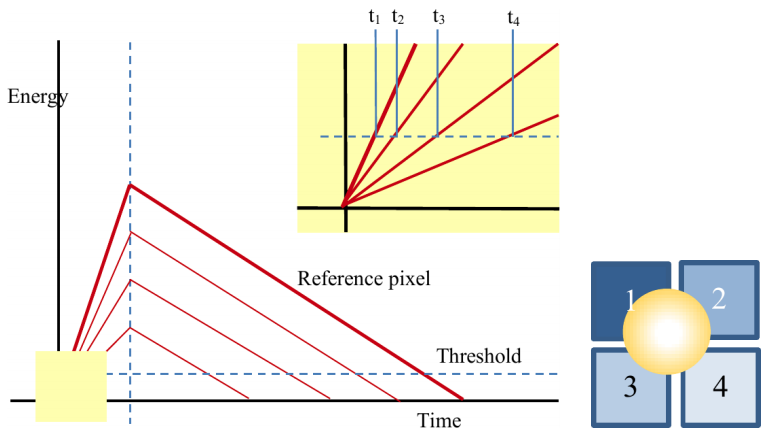
\includegraphics[width=12cm]{figures/calib_timeWalk.png}
		\caption{\textit{Time-walk} efekt: příklad interakce jedné částice se čtyřmi pixely detektoru, kde v každém pixelu byla deponována jiná energie, což na výstupů zesilovačů pixelů způsobilo jiné hodnoty napětí. Díky rozdílné charakteristice náběžné hrany pulzů byl treshold překročen v různých časech ($t_{1-4}$) \cite{Turecek2016TimeWakl}.}
		\label{fig:det:calib:timeWalk}
	\end{center}
\end{figure}

S použitím detektoru \textit{Timepix3}\cite{timepix3} je možné tuto energeticky závislou chybu eliminovat za použití kalibrační metody \cite{Turecek2016TimeWakl}, protože tento detektor umožňuje měřit v ToA a ToT módu současně. Tato kalibrační metoda spočívá v analytickém zpracování dat získaných z měření se zdrojem alfa částic (v \cite{Turecek2016TimeWakl} použito $^{241}$\texttt{Am}), které generuje clustery o velikosti maximálně čtyři pixely. Nejprve je však třeba potřeba energeticky zkalibrovat \ref{chap:detectors:calibration:energy}. 

O vybraných clusterech o velikosti 3 a 4 pixely pro $^{241}$\texttt{Am} víme, že součet jejich energií je $59.5keV$. Z clusteru je vybraný pixel s energií $30keV$, který je použit jako referenční (na \ref{chap:detectors:calibration:timeWalk} jako $t_1$), zbylá energie je náhodně rozdělena mezi ostatní pixely (na \ref{chap:detectors:calibration:timeWalk} jako $t_{2-4}$). Jednotlivé rozdíly $t_i+t_1$ jsou analytickými metodami, popsanými v \cite{Turecek2016TimeWakl}, zpracovány a výsledkem tohoto procesu jsou konstanty $c,d$ pro každý pixel detektoru, kterými lze vypočítat jeho \textit{Time-Walk offset} $\Delta T$:

\begin{equation}\label{eq:det:timeWalk}
	\Delta T = \frac{c}{(E - E_0)^d}
\end{equation}
kde:
\begin{changemargin}{1.5cm}{1cm} 
	\begin{itemize}
		\item [$\Delta T$] je \textit{Time-Walk} korekce pixelu [$ns$] (výsledná hodnota ToA je pak rovna $ToA-\Delta T$),
		\item [$E$] je energie pixelu [keV],
		\item [$E_0$] je treshold pixelu [keV] a
		\item [$c,d$] jsou konstanty.
	\end{itemize}
\end{changemargin}